\section{Introduzione}
L'equazione di diffusione in un corpo bidimensionale \`e
\[
	u_t= D(u_{xx}+ u_{yy} +f)
\]
mentre in un corpo a tre dimensioni (solido) \`e
\[
	u_t=D\left( u_{xx}+u_{yy} +u_{zz} \right) +f
\]
L'operatore
\[
	\Delta= \partial_{x_1x_1}+ \ldots + \partial_{x_n x_n}
\]
in ogni dimensione $n$ \`e detto \textit{Laplaciano}. Con questa notazione
l'equazione di diffusione si scrive
\[
	u_t= D\Delta u +f
\]
Nel caso di sorgenti $f$ non dipendenti dal tempo, \`e ragionevole cercare
soluzioni stazionarie, cio\`e anch'esse indipendenti da $t$.
Si giunge cos\`i all'\textit{equazione di Poisson}
\[
	\Delta u= -f/D
\]
Nel caso omogeneo $f=0$, l'equazione
\[
	\Delta u=0
\]
si dice \textit{equazione di Laplace} e le soluzioni si dicono
\textit{funzioni armoniche}.\\
Anche le soluzioni stazionarie dell'equazione
\[
	u_{tt}c^2 \Delta u
\]
sono funzioni armoniche. In dimensione di spazio $n=2$, questa equazione
descrive lo spostamento di una membrana elastica dalla posizione di riposo.
Una posizione stazionaria (equilibrio) \`e quindi descritta da una funzione
armonica.
Se $F=(f_1,f_2, f_3)=f_1= f_1 \uvi + f_2 \uvj + f_3 \uvk$ \`e un campo
vettoriale nello spazio, la divergenza di $F$ \`e lo scalare
\[
	div F= \partial_x f_1 + \partial_y f_2 + \partial_z f_3
\]
Se esiste una funzione scalare $u$ tale che
\[
	\nabla u= F
\]
(potenziale), allora
\[
	div F= div \nabla u = div \left( u_x \uvi +u_y \uvj + u_x \uvk \right)
	=\Delta u
\]
L'equazione di Laplace/Poisson \`e quindi fondamentale nello studio dei campi
conservativi. Se $E$ \`e un campo elettrostatico in una regione $\Omega$
di spazio, allora si ha
\[
	div E= \frac{4 \pi \rho}{\varepsilon}
\]
con $\rho$ densit\`a di carica ed $\varepsilon$ costante dielettrica. Se
\[
	\Delta u= -E
\]
il potenziale soddisfa l'equazione di Poisson
\[
	\Delta u= - \frac{4 \pi \rho}{\varepsilon}
\]
Nel caso $\rho=0$, cariche fuori di $\Omega$, la funzione $u$ \`e armonica.
In dimensione $n=2$, le funzioni armoniche intervengono anche nello studio
di funzioni di variabile complessa.
Se $f= u+iv$ \`e derivabile in senso complesso, vale l'equazione di
Cauchy- Riemann
\[
	\frac{\partial f}{\partial x}= \frac{1}{i} \frac{\partial f}
	{\partial y}
\]
che si scrive anche
\[
	\left\{
	\begin{array}{l}
		u_x=v_y \\
		v_x=- u_y
	\end{array}
	\right.
\]
Dunque
\[
	\Delta u= u_{xx}+ u_{yy}= v_{yx}-v_{xy}=0
\]
\[
	\Delta v= v_{xx}+ v_{yy}= -u_{yx} +u_{xy}=0
\]
La parte reale $u$ e l parte immaginaria $v$ di $f$ sono funzioni
armoniche.
Viceversa, se $u$ \`e una funzione armonica, \`e possibile risolvere le
equazioni di Cauchy-Riemann rispetto a $v$ in ogni parte semplicemente connessa
del dominio in modo che
\[
	f= u+ iv
\]
sia una funzione derivabile in senso complesso.
Tale funzione \`e in realt\`a derivabile infinite volte perch\'e si pu\`o
espandere localmente in serie di potenze. Ne segue che $u$ (e $v$) \`e
derivabile infinite volte in $dx$, $dy$.
Abbiamo cos\`i che una funzione armonica nel piano \`e derivabile infinite
cio\`e di classe $C^{\infty}$.
\section{Formule di Gauss-Green ed applicazioni al Laplaciano}
Se $\gamma$ \`e una curva chiusa nel piano, orientata in senso antiorario,
regolare (a tratti) con parametrizzazione
\[
	x= x(t), \;\;\; y=y(t), \;\;\; a\leq t \leq b
\]
Il versore tangente a $\gamma$
\[
	{\bf T}= \frac{1}{\sqrt{(x')^2+ (y')^2}}(x', y')
	=\frac{x'}{\sqrt{(x')^2+ (y')^2}}\uvi
	+\frac{y'}{\sqrt{(x')^2+ (y')^2}}\uvj
\]
Ora, per ottenere il versore normale ${\bf N}$, bisogna calcolare il versore
ortogonale a ${\bf T}$; ci\`o \`e ottenuto con
\[
	{\bf N}= \frac{1}{\sqrt{(x')^2+ (y')^2}}(y', -x')
	=\frac{y'}{\sqrt{(x')^2+ (y')^2}}\uvi
	-\frac{x'}{\sqrt{(x')^2+ (y')^2}}\uvj
\]
che rappresenta la normale esterna a $\gamma$; la normale interna \`e invece
\[
	{\bf N}= \frac{1}{\sqrt{(x')^2+ (y')^2}}(-y', x')
	=-\frac{y'}{\sqrt{(x')^2+ (y')^2}}\uvi
	+\frac{x'}{\sqrt{(x')^2+ (y')^2}}\uvj
\]
Dato un campo vettoriale $F= f_1 \uvi + f_2 \uvj$, gli integrali curvilinei
\[
	\int_ {\gamma} F \cdot {\bf T} ds=
	\int_a^b \left[ f_1 (x(t), y(t))x'(t)+
	f_2 (x(t), y(t))y'(t)
	\right] dt
\]
\[
	\int_ {\gamma} F \cdot {\bf N} ds=
	\int_a^b \left[ f_1 (x(t), y(t))y'(t)
	- f_2 (x(t), y(t))x'(t)
	\right] dt
\]
rappresentano, rispettivamente, il lavoro di $F$ su $\gamma$ ed il flusso
uscente di $F$ da $\Omega$. Si \`e fatto uso dello spostamento infinitesimo
\[
	ds= \sqrt{(x')^2+(y')^2}
\]

Le formule di Gauss-Green collegano gli integrali curvilinei su $\gamma$
ad integrali in $dx dy$ su $\Omega$:
\[
	\int_{\Omega}\partial_x f(x,y)dx dy= \int_{\gamma} f \uvj \cdot {\bf T}
ds
\]
\[
	\int_{\Omega}\partial_y f(x,y)dx dy= - \int_{\gamma} f \uvi \cdot {\bf
T} ds
\]
Tali formule sono di facile dimostrazione su domini normali. Ad esempio
preso $\Omega$ come in fig. \ref{nor_dom}
\begin{figure}[H]
	\centering
	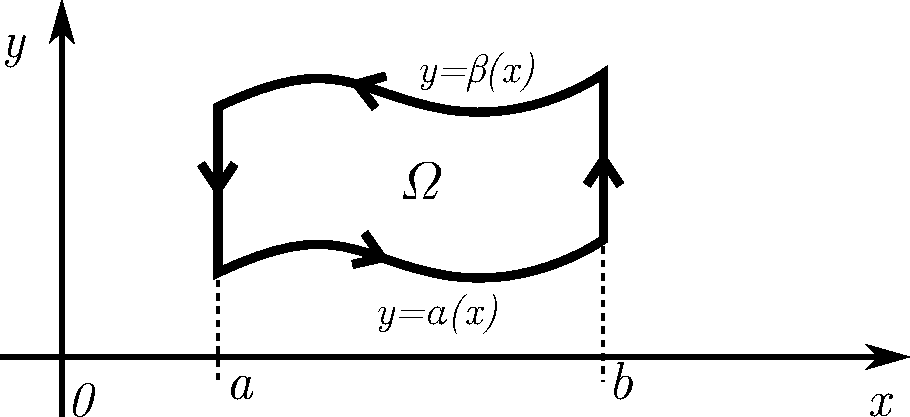
\includegraphics[width=0.8\textwidth]{nor_dom.pdf}
	\caption{Dominio normale per la dimostrazione delle formule di Green.}
	\label{nor_dom}
\end{figure}
\noindent
si ha
\[
	\int_{\Omega} \partial_y f (x,y) dx dy=
	\int_a^b \int_{\alpha(x)}^{\beta(x)}
	\partial_y f (x,y) dx dy=
	\int_a^b \left[
		f(x,y)
	\right]_{y=\alpha(x)}^{y=\beta(x)}dx
\]
\[
	= \int_a^b \left[
	f(x,\beta (x)) - f(x, \alpha(x))
	\right] dx
\]
Per il tratto di frontiera
\[
	\left\{
	\begin{array}{ll}
		x=x & x \in [a,b] \\
		y= \alpha(x)
	\end{array}
	\right.
\]
si ha
\[
	{\bf T}= \frac{1}{\sqrt{1+ (\alpha ' )^2}}(1,\alpha ')
\]
\[
	ds= \sqrt{1+ (\alpha ' )^2} dx
\]
\[
	{\bf T} \cdot \uvi ds= dx
\]
perci\`o
\[
	\int \limits_{\gamma_{[a,b]}} f(x,y)\uvi \cdot {\bf T} ds
	= \int_a^b f(x, \alpha(x)) dx
\]
Per il tratto orientato in senso contrario
\[
	\left\{
	\begin{array}{ll}
		x=x & x \in [b,a] \\
		y= \beta(x)
	\end{array}
	\right.
\]
si ha
\[
	{\bf T}= - \frac{1}{\sqrt{1+ (\beta ' )^2}}(1,\beta ')
\]
\[
	ds= \sqrt{1+ (\beta ' )^2} dx
\]
\[
	{\bf T} \cdot \uvi ds= -dx
\]
perci\`o
\[
	\int \limits_{\gamma_{[b,a]}} f(x,y)\uvi \cdot {\bf T} ds
	= \int_b^a f(x, \beta(x)) dx
	= -\int_a^b f(x, \beta(x)) dx
\]
Nei due tratti verticali si ha ${\bf T} = \pm \uvj$,
quindi ${\bf T} \cdot \uvi = 0$.\\
Per concludere
\[
	\int_{\gamma} f(x,y)\uvi \cdot {\bf T} ds =
	\int_a^b f(x, \alpha(x)) dx
	- \int_a^b f(x, \beta(x)) dx=
\]
\[
	- \int_a^b \left[ f(x, \beta(x)) -f(x, \alpha(x)) \right] dx
\]
e quindi
\[
	\int_{\gamma} f(x,y)\uvi \cdot {\bf T} ds =
	- \int_{\Omega} \partial_y f (x,y) dx dy=
\]
Il teorema diventa estendibile anche a domini non normali, data la possibilit\`a
di scomporre un dominio qualsiasi in domini normali.

Analoga dimostrazione pu\`o essere fatta per la formula restante, in questo
caso utilizzando un dominio perpendicolare all'asse y.

Per un campo $F= f_1 \uvi + f_2 \uvj$ si ottiene
\[
	\int_{\gamma} F \cdot {\bf T} ds
	= \int_{\gamma} f_1 \uvi \cdot {\bf T} ds
	+ \int_{\gamma} f_2 \uvj \cdot {\bf T} ds
	= \int_{\Omega} (\partial_x f_2 - \partial_y f_1)dxdy
\]
cio\`e la formula di Stokes
\[
	\int_{\gamma} F \cdot {\bf T} ds
	= \int_{\Omega} (\partial_x f_2 - \partial_y f_1)dxdy
\]
nel piano. L'integrale doppio pu\`o essere visto come il flusso attraverso la
superficie piana $\Omega$ di $rot F$ pensando ad $F= f_1 \uvi + f_2 \uvj +0\uvk$
nello spazio.\\
Inoltre, ricordando che
\[
	{\bf N} \cdot \uvi= {\bf T} \cdot \uvj, \;\;\;
	{\bf N} \cdot \uvj= -{\bf T} \cdot \uvi
\]
si ha
\[
	\int_{\gamma} F \cdot {\bf N} ds=
	\int_{\gamma} f_1 \uvi \cdot {\bf N} ds +
	\int_{\gamma} f_2 \uvj \cdot {\bf N} ds =
	\int_{\gamma} f_1 \uvj \cdot {\bf T} ds -
	\int_{\gamma} f_2 \uvi \cdot {\bf T} ds =
\]
\[
	\int_{\Omega} \left( \partial_x f_1 + \partial_y f_2 \right)dxdy
\]
che \`e il teorema della divergenza nel piano
\[
	\int_{\gamma} F \cdot {\bf N} ds=
	\int_{\Omega} div F \; dxdy
\]
Le formule di Gauss-Green e le loro conseguenze forniscono importati
applicazioni
al Laplaciano.

Per $F= \nabla u$, il teorema della divergenza diventa
\[
	\int_{\Omega} \Delta u \; dxdy=
	\int_{\gamma} \nabla u \cdot {\bf N} ds =
	\int_{\gamma} \partial_{\bf N} u \; ds
\]
in quanto $\nabla u \cdot {\bf N}$ coincide con la derivata
$ \partial_{\bf N} u$ lungo la normale esterna.\\
Applicando poi il teorema della divergenza al campo
\[
	vF= vf_1 \uvi + vf_2 \uvj
\]
si ha
\[
	div(vF)= v_x f_1 + v_y f_2 +
	v \left( \frac{\partial}{\partial_x} f_1
	+ \frac{\partial}{\partial_y} f_2 \right)
\]
\[
	= \nabla v \cdot F + v\, divF
\]
perci\`o
\[
	\int_{\gamma} vF \cdot {\bf N} ds =
	\int_{\Omega} div(vF) \; dxdy=
	\int_{\Omega} \nabla v \cdot F \; dxdy +
	\int_{\Omega} v\, divF \; dxdy
\]
Questa, con $F= \nabla u$, si riduce a
\[
	\int_{\gamma} v \, \partial_{\bf N} u \; ds =
	\int_{\Omega} \nabla v \cdot \nabla u \; dxdy +
	\int_{\Omega} v\, \Delta u \; dxdy
\]
che conviene mettere nella forma di integrale per parti per il Laplaciano
\[
	\int_{\Omega} v\, \Delta u \; dxdy =
	\int_{\gamma} v \, \partial_{\bf N} u \; ds -
	\int_{\Omega} \nabla v \cdot \nabla u \; dxdy
\]
\section{Problemi ben posti}
Sia $\Omega$ un dominio limitato di $\mathbb{R}^2$ con frontiera $\gamma$
curva chiusa regolare a tratti orientata in senso positivo.
I problemi ben posti per l'equazione $\Delta u= f$ in $Omega$ sono quelli
visti per la diffusione, senza dato iniziale mancando la variabile tempo.\\
Per il problema di Dirichlet:
\[
	\left\{
	\begin{array}{ll}
		\Delta u= f & \text{in} \;\;\; \Omega \\
		u= g & \text{in} \;\;\; \gamma
	\end{array}
	\right.
\]
Per il problema di Neumann:
\[
	\left\{
	\begin{array}{ll}
		\Delta u= f & \text{in} \;\;\; \Omega \\
		\partial_{\bf N}u= h & \text{in} \;\;\; \gamma
	\end{array}
	\right.
\]
La formula
\[
	\int_{\Omega} \Delta u \; dxdy=
	\int_{\gamma} \partial_{\bf N} u \; ds
\]
fornisce una condizione di compatibilit\`a tra la sorgente $f$ ed il flusso
uscente $h$ nel problema di Neumann. La condizione necessaria per l'esistenza
di soluzioni \`e
\[
	\int_{\Omega} f \; dxdy=
	\int_{\gamma} h \; ds
\]

\section{Unicit\`a}
Si mostra che i problemi con dati iniziali coincidenti hanno la stessa
soluzione.\\
Se $u_1$ $u_2$ sono due soluzioni allora
\[
	w=u_1- u_2
\]
risolve
\[
	\Delta w = 0 \;\;\; \text{in} \;\;\; \Omega
\]
con condizioni al contorno
\[
	\begin{array}{lll}
		w=0 & \text{in } \gamma & \text{Dirichlet}\\
		\partial_{\bf N}w=0 & \text{in } \gamma & \text{Neumann}\\
	\end{array}
\]
Sostituendo $u=v=w$ nella formula dell'integrale per parti
(equivalente ad usare il campo $div\, (ww)= div\, w^2$)
\[
	\int_{\Omega} w \Delta w \, dxdy=
	- \int_{\Omega} \nabla w \cdot \nabla w \, dxdy
	+ \int_{\gamma} w \partial_{\bf N} w \, ds
\]
il termine
\[
	\int_{\gamma} w \partial_{\bf N} w \, ds
\]
\`e nullo sia con condizioni di Neumann nulle ($\partial_{\bf N} w =0 $) sia
con le condizioni di Dirichlet nulle ($w=0$).
Perci\`o, data la definizione $\Delta w= 0$,
\[
	0= - \int_{\Omega} \left|\left| \nabla w \right|\right|^2 \, dxdy +0
\]
\[
	\int_{\Omega} \left|\left| \nabla w \right|\right|^2 \, dxdy = 0
\]
L'unica soluzione, essendo somma di quadrati, \`e
\[
	\nabla w=0
\]
in $\Omega$. Quindi
\[
	w=C \;\;\; \text{in} \;\;\; \Omega
\]
Questo pone l'unicit\`a a meno di costanti nel caso di Neumann.\\
Per Dirichlet deve essere $w=c=0$ in $\gamma$ (o almeno $\gamma_0$),
quindi $w=0$ ovunque nella chiusura $\bar{\Omega}= \Omega \cup \gamma$ di
$\Omega$.
\section{Propriet\`a di media}
Sia $u(x,y)$ armonica in $\Omega \leq \mathbb{R}^2$
\[
	\Delta u= 0 \;\;\; \text{in} \;\;\; \Omega
\]
Denotiamo con $\Omega_R(x,y)$ un generico cerchio di centro $(x,y)$ e raggio
$R$ contenuto in $\Omega$ e con $\gamma_R(x,y)$ la circonferenza di frontiera
orientata positivamente.
\begin{figure}[H]
	\centering
	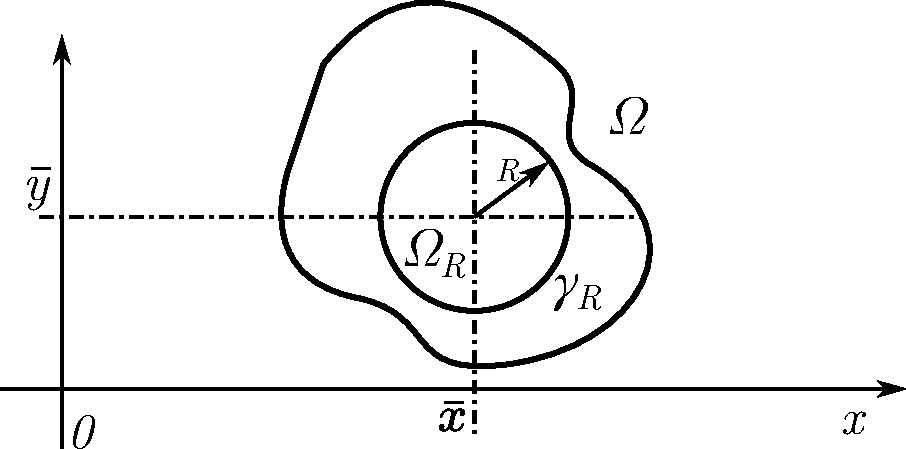
\includegraphics[width=0.8\textwidth]{mean_f.pdf}
	\caption{Circonferenza di frontiera $\gamma_R$.}
	\label{mean_f}
\end{figure}
\noindent
\subsection{Formule di media}
In tale dominio circolare valgono le formule di media
\[
	u(\bar{x}, \bar{y})= \frac{1}{\pi R^2}
	\int \limits_{\Omega_R}
	u(x,y) \, dxdy
\]
\[
	u(\bar{x}, \bar{y})= \frac{1}{2 \pi R}
	\int \limits_{\gamma_R}
	u \, ds
\]
con $ds$ l'elemento di lunghezza sulla circonferenza.
\subsubsection{Dimostrazione}
Iniziamo dalla seconda. Per $0<\pi<R$ poniamo
\[
	g(r)= \frac{1}{2\pi r}
	\int \limits_{\gamma_r}
	u \, ds=
	\frac{1}{2\pi r}
	\int_0^{2\pi}
	u(\bar{x}+rcos \theta, \bar{y} + rsin \theta) \, r d\theta
\]
\[
	= \frac{1}{2\pi}
	\int_0^{2\pi}
	u(\bar{x}+rcos \theta, \bar{y} + rsin \theta) \, d\theta
\]
dove si \`e usata la parametrizzazione di $\gamma_r(x,y)$
\[
	\left\{
		\begin{array}{l}
			x= \bar{x} + rcos\theta \\
			y= \bar{y} + rsin\theta
		\end{array}
	\right.
\]
con $0 \leq \theta \leq 2\pi$.\\
Dove $x'=-rsin \theta$, $y'= rcos \theta$, $ds= \sqrt{(x')^2+ (y')^2}=
rd\theta$.\\
Derivando $g(r)$ abbiamo
\[
	g'(r)= \frac{1}{2\pi}
	\int_0^{2\pi}
	\left(
		u_x cos\theta + u_y sin \theta
	\right)d\theta=
	\frac{1}{2\pi r}
	\int \limits_{\gamma_r} \nabla u \cdot {\bf N} ds
\]
dove si \`e usato
\[
	{\bf N} = cos\theta \uvi + sin \theta \uvj , \;\;\;
	d\theta= \frac{ds}{r}
\]
Per il teorema della divergenza
\[
	\frac{1}{2\pi r}
	\int \limits_{\gamma_r} \nabla u \cdot {\bf N} ds=
	\int \limits_{\Omega_r} div (\nabla u) dxdy=
	\int \limits_{\Omega_r} \Delta u \, dxdy= 0
\]
cio\`e $g(r)$ costante.\\
Poich\'e
\[
	\lim_{r \to 0} g(r)=
	\lim_{r \to 0} \frac{1}{2 \pi}
	\int_0^{2\pi}
	u(\bar{x}+rcos \theta, \bar{y} + rsin \theta) \, d\theta=
	\frac{1}{2 \pi} \int_0^{2\pi}
	u(\bar{x}, \bar{y}) d\theta
\]
\[
	= u(\bar{x}, \bar{y})
\]
abbiamo
\[
	g(r)= u(\bar{x}, \bar{y}) \;\;\; \text{per ogni} \;\;\; r \in (0,R]
\]
il ch\'e prova la formula di media voluta.\\
Da questa si ottiene anche l'altra. Infatti da
\[
	u(\bar{x}, \bar{y})=
	\frac{1}{2 \pi} \int_0^{2 \pi}
	u(\bar{x}+rcos \theta, \bar{y} + rsin \theta) \, d\theta
\]
moltiplicando per $r$ ed integrando in $dr$ tra $0$ e $R$, segue
\[
	u(\bar{x}, \bar{y})\int_0^R rdr=
	\frac{1}{2\pi}\int_0^R
	\int_0^{2\pi}
	u(\bar{x}+rcos \theta, \bar{y} + rsin \theta) \, rd\theta dr
\]
\[
	u(\bar{x}, \bar{y})\frac{R^2}{2}=
	\frac{1}{2\pi} \int \limits_{\Omega_R} u(x,y) \, dxdy
\]
con $rdrd\theta= dxdy$.\\
Da cui
\[
	u(\bar{x}, \bar{y})=
	\frac{1}{\pi R^2}
	\int \limits_{\Omega_R} u(x,y) \, dxdy
\]
Queste ci dicono che i valori delle funzioni armoniche sono molto rigide.
Per calcolare la $u$ nel centro, sapendo che \`e armonica, basta avere i
valori sul bordo (del cerchio!).\\
Vedremo che, viceversa, una funzione che soddisfa la propriet\`a di media \`e
armonica. Da questa equivalenza seguir\`a poi che ogni funzione armonica \`e
$C^{\infty}$.
\subsection{Principi di massimo}
Una funzione che soddisfa la propriet\`a di media in $\Omega$ che non sia
una funzione costante non pu\`o avere massimi o minimi globali interni ad
$\Omega$.
Per vedere questo, basta vedere che se $u(x,y)$ in $\Omega$ assume valore
minimo (massimo) assoluto in $(\bar{x}, \bar{y})$ interno ad $\Omega$,
allora \`e costante in ogni cerchio $\Omega_R(\bar{x}, \bar{y})\subset \Omega$.
Se vale questo, infatti, tutti i punti di $\Omega_R(\bar{x}, \bar{y})$ diventano
di minimo (massimo) assoluto.
Il centro $(\bar{x}, \bar{y})$ pu\`o essere sostituito dai punti arbitrariamente
vicini al bordo di $\Omega_R(\bar{x}, \bar{y})$ e la regione dove $u$ \`e
costante
pu\`o essere allargata.
Con questo procedimento si giunge a far vedere che $u$ \`e costante su tutto
l'aperto e connesso $\Omega$.
\subsubsection{Teorema}
La  funzione $u$ soddisfi le propriet\`a di media in $\Omega$.
Se $u(\bar{x}, \bar{y})=m$ \`e minimo assoluto allora $u(x,y)=m$ in tutti
i punti di $\Omega_R(\bar{x}, \bar{y})\subset \Omega$.
\subsubsection{Dimostrazione}
Supponiamo che $u(x,y)\geq m_1 > m$ in $\Omega_r (x_0, y_0)\subset \Omega_R
(\bar{x}, \bar{y})$.
Allora
\[
	m= u(\bar{x}, \bar{y})=
	\frac{1}{\pi R^2}
	\int \limits_{\Omega_R} u(x,y) dx dy
\]
\[
	= \frac{1}{\pi R^2} \left\{
	\int \limits_{\mathrlap{\Omega_R (\bar{x}, \bar{y}) - \Omega_r
(x_0,y_0)}}
	u(x,y) \, dxdy +
	\int \limits_{\mathrlap{\Omega_r (x_0,y_0)}}
	u(x,y) \, dxdy +
	\right\}
\]
\[
	\geq \frac{1}{\pi R^2} \left\{
	\int \limits_{\mathrlap{\Omega_R (\bar{x}, \bar{y}) - \Omega_r
(x_0,y_0)}}
	m \, dxdy \;\;\;\; + \;\;\;\;
	\int \limits_{\mathrlap{\Omega_r (x_0,y_0)}}
	m_1 \, dxdy
	\right\}
\]
\[
	= \frac{1}{\pi R^2} \left\{
	m \cdot \text{Area} \left( \Omega_R (\bar{x}, \bar{y}) - \Omega_r
(x_0,y_0) \right) +
	m_1 \cdot \text{Area} \left(\Omega_r (x_0,y_0) \right)
	\right\}
\]
\[
	= \frac{1}{\pi R^2} \left\{
	m (\pi R^2 - \pi r^2) + m_1 \pi r^2
	\right\}
\]
\[
	> \frac{1}{\pi R^2} \left\{
	m (\pi R^2 - \pi r^2) + m \pi r^2
	\right\} =
	\frac{1}{\pi R^2} m\pi R^2 = m
\]
Siamo all'assurdo
\[
	m>m
\]
La funzione $u$ non pu\`o assumere valori $m_1>m$ all'interno di
$\Omega_R(\bar{x}, \bar{y})$.
Analogo risultato vale per i punti di massimo.
\subsubsection{Teorema}
La funzione $u$ soddisfi la propriet\`a di media nell'aperto connesso $\Omega$.
se $u$ ha minimo o massimo assoluti interni ad $\Omega$, allora $u$ \`e costante
in $\Omega$.
\subsubsection{Lemma}
Se $\Omega$ \`e limitato ed $u$ \`e continua nella chiusura $\bar{\Omega}$,
allora ha certamente massimo e minimo assoluti in $\bar{\Omega}$ per il
teorema di Weierstrass. Questi valori non possono essere assunti nei punti
interni, a meno che non sia costante, quindi sono assunti sulla frontiera.

\subsubsection{Teorema}
Se $u$ \`e continua in $\bar{\Omega}$ con $\Omega$ aperto, connesso e limitato
e soddisfa la propriet\`a di media in $\Omega$, allora
\[
	\max_{\bar{\Omega}} u= \max_{\gamma} u, \;\;\;
	\min_{\bar{\Omega}} u= \min_{\gamma} u
\]
\[
	\Downarrow
\]
\[
	\max_{\bar{\Omega}} |u|= \max_{\gamma} |u|
\]
con $\gamma$ la frontiera di $\Omega$.\\
Qualitativamente, l'unico punto in cui l'eventuale $u(\bar{x}, \bar{y})$ pu\`o
essere massimo o minimo \`e sulla frontiera, dove $\gamma_r$ ha diametro
infinitesimo e il valore all'interno di $\gamma_r$ pu\`o essere considerato
costante. In tutti gli altri casi deve essere sulla frontiera di $\gamma_r$;
perci\`o preso il dominio $\bar{\Omega}$, i minimi e massimi possono essere solo
sulla frontiera.
\section{Unicit\`a e dipendenza continua dai dati}
Presa una funzione armonica, essa soddisfa la propriet\`a di media.
Attraverso di essa possiamo dedurre un risultato di unicit\`a e dipendenza
continua dai dati per il problema di Dirichlet, senza ipotesi di regolarit\`a
sulla frontiera ed assumendo che $u$ sia solo continua in $\bar{\Omega}$.
\subsubsection{Teorema}
Sia $\Omega$ aperto, connesso e limitato in $\mathbb{R}^2$ e sia $g$ continua
nella frontiera $\gamma$ di $\Omega$.
Il problema
\[
	\begin{array}{ll}
		\Delta u= 0 & \text{in }\Omega \\
		u= g & \text{in }\gamma \\
	\end{array}
\]
ha al pi\`u una soluzione $u \in C^2 (\Omega) \cap C(\bar{\Omega})$
Inoltre, se $u_g$ indica la soluzione corrispondente al dato $g$, si ha
\[
	\max_{\bar{\Omega}} \left| u_{g_1} - u_{g_2} \right|=
	\max_{\gamma} \left| g_1 - g_2 \right|
\]
\subsubsection{Dimostrazione}
La funzione $u_{g_1} - u_{g_2}$ \`e armonica in $\Omega$ e continua in
$\bar{\Omega}$.\\
$\left| u_{g_1} - u_{g_2} \right|$ ha massimo in $\bar{\Omega}$, assunto sulla
frontiera $\gamma$. \\ Dunque
\[
	\max_{\bar{\Omega}} \left| u_{g_1} - u_{g_2} \right|=
	\max_{\gamma} \left| u_{g_1} - u_{g_2} \right|=
	\max_{\gamma} \left| g_1 - g_2 \right|
\]
poich\'e $u_g$ in $\gamma$ \`e uguale a $g$.\\
Il risultato precedente dimostra la dipendenza continua dai dati.
Ora se $g_1=g_2$ allora da questo segue $g_1=g_2$ in $\bar{\Omega}$, cio\`e
l'unicit\`a della soluzione.
\section{Esistenza della soluzione}
I teoremi di esistenza sono pi\`u difficili di quelli di unicit\`a.
I lcaso pi\`u semplice \`e quello di $\Omega$ cerchio nel piano dove si
possono utilizzare le coordinate polari. \`E quindi necessario procurarsi
l'espressione di $\Delta$ in queste coordinate.
\footnote{Vedi anche
\url{http://www1.mate.polimi.it/~bramanti/corsi/archivio_pdf/laplaciano.pdf}}
\subsection{Laplaciano in coordinate polari}
Per $u(r(x,y), \theta (x,y))$, ricordando che
\[
	\partial_x r= \partial_x\sqrt{x^2 + y^2}=\frac{x}{\sqrt{x^2 + y^2}}= cos
\theta
\]
\[
	\partial_y r= \partial_y\sqrt{x^2 + y^2}=\frac{y}{\sqrt{x^2 + y^2}}= sin
\theta
\]
\[
	\partial_x \theta= \partial_x arctan \frac{y}{x}=
	\frac{1}{1 +\frac{y^2}{x^2}} \left( - \frac{y}{x^2} \right)
\]
\[
	\partial_y \theta= \partial_y arctan \frac{y}{x}=
	\frac{1}{1 +\frac{y^2}{x^2}} \; \frac{1}{x}
\]
si ha
\[
	\partial_x u= cos \theta \partial_r u - \frac{sin \theta}{r}
\partial_{\theta} u
\]
\[
	\partial_y u= sin \theta \partial_r u + \frac{cos \theta}{r}
\partial_{\theta} u
\]
Calcolando
\[
	\partial_x^2 u = \partial_x(\partial_x u)=
	\left( cos \theta \partial_r  - \frac{sin \theta}{r} \partial_{\theta}
\right)
	\left( cos \theta \partial_r u - \frac{sin \theta}{r} \partial_{\theta}
u \right)
\]
ed eseguendo tutte le derivate e sommando si arriva a
\[
	\Delta u = \partial^2_r u + \frac{1}{r} \partial_r u
+\frac{1}{r^2}\partial^2_{\theta} u
\]
\subsection{Formula di Poisson}
Risolviamo quindi il problema di Dirichlet nel cerchio
\[
	\left\{
	\begin{array}{ll}
		\Delta u=0 	& \text{in } \Omega_R(\bar{x}, \bar{y}) \\
		u=g 		& \text{in } \gamma_R(\bar{x}, \bar{y})
	\end{array}
	\right.
\]
Col metodo della \textit{separazione delle variabili} in coordinate polari
\[
	\begin{array}{ll}
		x= \bar{x} + rcos \theta & 0 \leq \theta \leq 2 \pi \\
		y= \bar{y} + rsin \theta & 0 \leq r \leq R
	\end{array}
\]
poniamo
\[
	u= v(r)w(\theta)
\]
dove $w(\theta)$ deve essere periodica di periodo $2 \pi$.
\[
	\Delta u = 0
\]
\[
	\Downarrow
\]
\[
	v''(r)w(\theta)+ \frac{1}{r^2}v(r)w''(\theta)+
\frac{1}{r}v'(r)w(\theta)=0
\]
da cui, dividendo per $u= v(r)w(\theta)$ e moltiplicando per $r^2$
\[
	r^2 \frac{ v''(r)}{v(r)} + r \frac{v'(r)}{v(r)}=
	-\frac{w''(\theta)}{w(\theta)}
\]
Le due funzioni possono coincidere solo se costanti
\[
	- \frac{w''(\theta)}{w(\theta)}= k =
	r^2 \frac{ v''(r)}{v(r)} + r \frac{v'(r)}{v(r)}
\]
Inizialmente
\[
	w''(\theta)+ kw(\theta) =0
\]
\[
	\lambda^2 + k=0, \follows \lambda^2 = -k
\]
che ha soluzioni periodiche solo se $k > 0$.
In questo caso
\[
	\lambda= \pm i\sqrt{k}
\]
e
\[
	w= Acos(\sqrt{k} \theta)+ Bsin(\sqrt{k} \theta)
\]
Essa deve necessariamente avere periodo $2\pi$, cio\`e equivalente al periodo
del cerchio che delimita il dominio (effettivamente dopo un giro \`e sempre
la stessa soluzione).
Il periodo indicato si ha solo per $\sqrt{k}= 0,1,2,\ldots$, quindi
$k= 0,1,4, \ldots$ in particolare $k=m^2$ con $m \in \mathbb{N}+\{0\}$.
Abbiamo ottenuto le soluzioni
\[
	w_m= A_m cos (m\theta)+ B_m sin (m \theta), \;\;\; m=1,2,3,\ldots
\]
\[
	w_0= A_0/2= \text{ costante } (m=0)
\]
Risolviamo ora
\[
	r^2 v''(r)+ rv'(r)- m^2 v(r)=0
\]
Si tratta di una \textit{Equazione di Eulero} (l'esponente eguaglia il grado
della derivata) e si riduce ad una a coefficienti costanti ponendo
\[
	v(r)= y(ln r), \;\;\; v'(r)= \frac{1}{r} y'(ln r)
\]
\[
	v''(r)= \frac{1}{r^2}y''(ln r) + \left( - \frac{1}{r^2} \right)y'(ln r)
\]
Si ottiene, sostituendo $t= ln r$
\[
	y''(t)- \cancel{y'(t)}+ \cancel{y'(t)} - m^2 y(t)=0
\]
\[
	y''(t) - m^2 y(t)=0
\]
che \`e effettivamente a coefficienti costanti.\\
L'equazione caratteristica
\[
	\lambda^2 - m^2=0 \follows \lambda= \pm m
\]
porta alle soluzioni linearmente indipendenti (tenuto conto che $m\geq 0$)
\[
	y_1(t)= e^{mt}, \;\;\; y_2(t)= e^{-mt}
\]
Ora ritorno alla variabile in r con la sostituzione $t= ln r$
\[
	v_1(r)= e^{m lnr}= r^m
\]
\[
	v_2(r)= e^{-m lnr}= r^{-m}
\]
La soluzione $v_2$ deve essere scartata perch\'e in $m=0$ diverge.
Resta quindi la sola soluzione $v_1=r^m$.\\
Abbiamo cos\`i ottenuto la famiglia di funzioni armoniche
\[
	u_m= A_m r^m cos(m \theta)+ B_m r^m sin (m \theta), \;\;\; u_0= A_0/2
\]
Per linearit\`a, se si pu\`o derivare sotto il segno di serie,
\[
	u= \frac{A_0}{2} + \sum_{m=1}^{\infty}
	A_m r^m cos(m \theta)+ B_m r^m sin (m \theta)
\]
\`e una soluzione di $\Delta u=0$ nel cerchio, con $A_m$, $B_m$ coefficienti
tali che $u$ sia ancora soluzione di $\Delta u= 0$ derivando termine a
termine.\\
Per $r=R$ deve essere $u=g$; la condizione si realizza con
\[
	u(R, \theta)= G(\theta)= g(\bar{x}+ Rcos \theta, \bar{y} + Rsin\theta)
\]
si scrive la serie di Fourier di $G$
\[
	G(\theta) \sim \frac{a_0}{2}+
	\sum_{m=1}^{\infty} a_m cos (m \theta) + b_m sin (m \theta)
\]
dove i coefficienti sono dati da
\[
	a_m = \frac{1}{\pi}
	\int_{0}^{2 \pi} G(\theta)cos(m \theta) d\theta \; , \;\;\;
m=0,1,2,\ldots
\]
\[
	b_m = \frac{1}{\pi}
	\int_{0}^{2 \pi} G(\theta)sin(m \theta) d\theta \; , \;\;\; m=1,2,\ldots
\]
Deve essere
\[
	A_0=a_0, \;\;\; A_m=\frac{a_m}{R^m}, \;\;\; B_m = \frac{b_m}{R^m}
\]
Con questa scelta si vede che per $g$ continua, la funzione
\[
	u=\frac{A_0}{2}+ \sum_{m=1}^{\infty} \left(
	A_mr^m cos (m \theta)+ B_m r^m sin (m \theta)
	\right)
\]
risolve
\[
	\left\{
	\begin{array}{ll}
		\Delta u=0 	& \text{in } \Omega_R(\bar{x}, \bar{y}) \\
		u=g 		& \text{in } \gamma_R(\bar{x}, \bar{y})
	\end{array}
	\right.
\]
Tale soluzione \`e in realt\`a $C^{\infty}$ all'interno di $\Omega_R (\bar{x},
\bar{y})$
e continua nel cerchio chiuso. Come gi\`a sappiamo, \`e l'unica soluzione.
Vogliamo ora semplificarne l'espressione. Per evitare incomprensioni con la
notazione, riscriviamo i coefficienti
\[
	A_m = \frac{1}{\pi R^m}
	\int_{0}^{2 \pi} G(\phi)cos(m \phi) d\phi
\]
\[
	B_m = \frac{1}{\pi R^m}
	\int_{0}^{2 \pi} G(\phi)sin(m \phi) d\phi
\]
Si ha, scambiando i simboli di serie e di integrale,
\[
	u= \frac{1}{\pi} \int_{0}^{2\pi} G(\phi)
	\left[
	\frac{1}{2}+ \sum_{m=1}^{\infty} \left( \frac{r}{R} \right)^m
	\left(
	cos(m \phi)cos(m \theta) + sin(m\phi)sin(m \theta)
	\right)
	\right] d\phi
\]
\[
	= \frac{1}{\pi} \int_{0}^{2\pi} G(\phi)
	\left[
	\frac{1}{2}+ \sum_{m=1}^{\infty} \left( \frac{r}{R} \right)^m
	cos (m(\phi - \theta))
	\right] d\phi
\]
Ora
\[
	cos(m(\phi - \theta))= {\mathcal Re}(e^{im(\phi - \theta)})
\]
quindi la serie vale, per $r>R$,
\[
	{\mathcal Re} \left(
	\sum_{m=1}^{\infty} \left( \frac{r}{R} e^{i(\phi - \theta)} \right)^m
	\right)
	=
	{\mathcal Re} \left(
	\frac{1}{1 - \frac{r}{R} e^{i(\phi - \theta)}}
	\right) -1
\]
\[
	= {\mathcal Re} \left(
	\frac{R}{R -rcos(\phi - \theta) - i \, rsin (\phi - \theta)}
	\right) -1
\]
razionalizzando
\[
	= {\mathcal Re} \left(
	\frac{R^2 - Rrcos(\phi - \theta) + i \, Rr sin (\phi - \theta)}
	{\left( R- rcos (\phi - \theta) \right)^2 + r^2 sin^2 (\phi - \theta)}
	\right) -1
\]
quindi
\[
	=\frac{R^2 - Rrcos(\phi - \theta)}
	{R^2 + r^2 -2Rrcos(\phi - \theta)}
	-1
\]
La soluzione si scrive
\[
	u= \frac{1}{\pi} \int_{0}^{2\pi} G(\phi)
	\left( \frac{1}{2}+
	\frac{Rrcos(\phi - \theta) -r^2}
	{R^2 + r^2 -2Rrcos(\phi - \theta)}
	\right)
	d\phi
\]
\[
	= \frac{1}{2 \pi} \int_{0}^{2\pi} G(\phi)
	\frac{R^2 + r^2 -\cancel{2Rrcos(\phi - \theta)} +
	\cancel{2Rrcos(\phi - \theta)} -2r^2 }
	{R^2 + r^2 -2Rrcos(\phi - \theta)}
	d\phi
\]
\[
	u = \frac{1}{2 \pi} \int_{0}^{2\pi} G(\phi)
	\frac{R^2 - r^2 }
	{R^2 + r^2 -2Rrcos(\phi - \theta)}
	d\phi
\]
I termini da infiniti sono diventati un termine singolo.\\
Torniamo alle variabili cartesiane
\[
	\left\{
	\begin{array}{ll}
		x= x(r, \theta)= \bar{x} + rcos \theta
		& \text{in } \Omega_R (\bar{x},\bar{y}) \\
		y= y(r, \theta)= \bar{y} + rsin \theta
	\end{array}
	\right.
\]
\[
	\left\{
	\begin{array}{ll}
		\sigma= \sigma(\phi)= \bar{x} + Rcos \phi
		& \text{in } \gamma_R (\bar{x},\bar{y}) \\
		\eta= \eta(\phi)= \bar{y} + Rsin \phi
	\end{array}
	\right.
\]
infatti con $r=R \follows \theta \longrightarrow \phi$ \\
la quantit\`a
\[
	R^2 + r^2 -2Rrcos(\phi - \theta) =
	\left( x(r, \theta)- \sigma (\phi) \right)^2 +
	\left( y(r, \theta)- \eta (\phi) \right)^2
\]
Attraverso il teorema del coseno\footnote{Vedi anche
\url{http://wikipedia.org/wiki/Law_of_cosines}
} (o di Carnot) oppure utilizzando le espressioni di
$x (r, \theta)$, $y(r, \theta)$, $\sigma (\phi)$, $\eta (\phi)$ (l'angolo
opposto ad $a$ \`e $\phi - \theta$)
\[
a^2= R^2 +r^2 -2Rrcos(\phi - \theta)
\]
\begin{figure}[H]
	\centering
	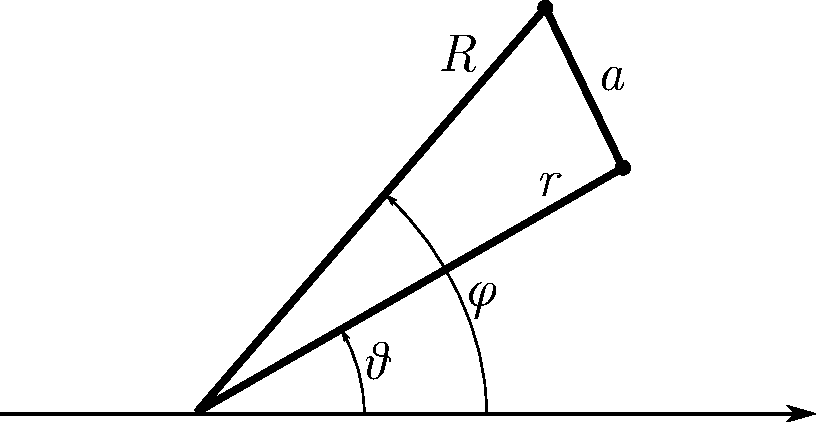
\includegraphics[width=0.6\textwidth]{car_th.pdf}
	\caption{Teorema di Carnot.}
	\label{car_th}
\end{figure}

L'elemento di lunghezza infinitesima in $\gamma_R (\bar{x}, \bar{y})$ \`e
\[
	ds= Rd\phi
\]
quindi si ottiene l'importante formula di Poisson
\[
	u(x,y)= \frac{r^2 - (x - \bar{x})^2 - (y -\bar{y})^2}{2 \pi R}
	\int_{\gamma_R} \frac{g(\sigma, \eta)}{(x - \sigma)^2+(y - \eta)^2} ds
\]
Provando con $(x,y)=(\bar{x},\bar{y})$ si ottiene la prima formula di media.
\[
	u (\bar{x},\bar{y}) = \frac{\cancel{R^2}}{2\pi R}
	\int_{\gamma_r} \frac{g}{\cancel{R^2}} ds=
	\frac{1}{2\pi R}
	\int_{\gamma_r} g ds=
\]
\subsubsection{Riassumendo}
Sia $g$ continua. L'unica soluzione
$u \in C^2 (\Omega_R (\bar{x}, \bar{y})) \cap C( \bar{ \Omega}_R (\bar{x},
\bar{y}))$ di
\[
	\left\{
	\begin{array}{ll}
		\Delta u=0 	& \text{in } \Omega_R(\bar{x}, \bar{y}) \\
		u=g 		& \text{in } \gamma_R(\bar{x}, \bar{y})
	\end{array}
	\right.
\]
\`e data da
\[
	u(x,y)= \frac{r^2 - (x - \bar{x})^2 - (y -\bar{y})^2}{2 \pi R}
	\int_{\gamma_R} \frac{g(\sigma, \eta)}{(x - \sigma)^2+(y - \eta)^2} \;
ds
\]
Tale soluzione \`e $C^{\infty}$ in $\Omega_R(\bar{x}, \bar{y})$.

\subsection{\texorpdfstring
{Le funzioni con propriet\`a di media sono armoniche e $\in C^{\infty}$}
{Le funzioni con propriet\`a di media sono armoniche e C inf}}
Abbiamo visto che le funzioni armoniche hanno la propriet\`a di media.
Vediamo ora che ogni funzione con propriet\`a di media \`e armonica e
$C^{\infty}$.
\subsubsection{Teorema}
Sia $u$ continua in $\Omega$ con la propriet\`a di media nei cerchi di
$\Omega$. Allora $u$ \`e armonica in $\Omega$ e $C^{\infty}$ in $\Omega$.\\
In particolare ogni funzione armonica \`e $C^{\infty}$.
\subsubsection{Dimostrazione}
Sia $\Omega_R(\bar{x}, \bar{y})$ un cerchio in $\Omega$ e consideriamo il
problema
\[
	\left\{
	\begin{array}{ll}
		\Delta v=0 	& \text{in } \Omega_R(\bar{x}, \bar{y}) \\
		v=u		& \text{in } \gamma_R(\bar{x}, \bar{y})
	\end{array}
	\right.
\]
La funzione \`e armonica quindi ha la propriet\`a di media come $u$.
La differenza $u-v$ ha la propriet\`a di media (linearit\`a dell'integrale)
quindi
\[
	\max_{\bar{\Omega}_R(\bar{x}, \bar{y})} |u-v|=
	\max_{{\gamma}_R(\bar{x}, \bar{y})} |u-v|
\]
per il principio di massimo di cui godono le funzioni con tale propriet\`a.
Sul bordo ${\gamma}_R(\bar{x}, \bar{y})$ si ha $u-v=0$ quindi $u=v$ anche in
$\Omega_R(\bar{x}, \bar{y})$.
La funzione $u$ \`e quindi armonica e $C^{\infty}$ in quanto si rappresenta
con la formula di Poisson in $\Omega_R(\bar{x}, \bar{y})$.
Per l'arbitrariet\`a di $\Omega_R(\bar{x}, \bar{y})$, ci\`o rimane vero in
tutto $\Omega$.
\subsection{L'equazione di Poisson}
Il metodo della separazione delle variabili si pu\`o applicare anche al
problema non omogeneo
\[
	\left\{
	\begin{array}{ll}
		\Delta u= f	& \text{in } \Omega_R(\bar{x}, \bar{y}) \\
		u=0		& \text{in } \gamma_R(\bar{x}, \bar{y})
	\end{array}
	\right.
\]
con $f$ funzione continua. Passiamo nelle coordinate polari e scriviamo
\[
	f(r, \theta)= f(\bar{x}+rcos \theta, \bar{y}+ rsin \theta)
\]
Per ogni $r \in (0,R)$, $f(r, \theta)$ \`e una funzione periodica di $\theta$
con $T=2\pi$. Si pu\`o quindi scrivere in serie di Fourier.
\[
	f(r,\theta)= 	\frac{a_0(r)}{2}+  \sum_{m=1}^{\infty} \left[
	a_m (r) cos (m \theta)+
	b_m(r) sin (m\theta)
	\right]
\]
Cerchiamo ora una soluzione dello stesso tipo
\[
	u(r,\theta)= 	\frac{A_0(r)}{2}+  \sum_{m=1}^{\infty} \left[
	A_m (r) cos (m \theta)+
	B_m(r) sin (m\theta)
	\right]
\]
dove in questo caso i coefficienti sono incognite.\\
Imponiamo, con il Laplaciano in coordinate polari, $\Delta u= f$ termine
a termine.
\[
	\Delta = \partial_r^2 +\frac{1}{r}\partial_r +
\frac{1}{r^2}\partial_{\theta}^2
\]
Si ottiene
\begin{align*}
	\Delta u = \frac{A_0''(r)+ \frac{1}{r}A_0'(r)}{2} &+
	\sum_{m=1}^{\infty} \left(
	A_m''(r) + \frac{1}{r} A_m'(r) -\frac{m^2}{r^2}A_m(r)
	\right)cos(m\theta) + \\
	&+ \sum_{m=1}^{\infty} \left(
	B_m''(r) + \frac{1}{r} B_m'(r) -\frac{m^2}{r^2}B_m(r)
	\right) sin (m\theta)
\end{align*}
eguagliando i vari termini per la serie
\[
	A_m'' + \frac{1}{r} A_m'-\frac{m^2}{r^2} A_m= a_m \;\;\;m=0,1,2,\ldots
\]
\[
	B_m'' + \frac{1}{r} B_m'-\frac{m^2}{r^2} B_m= b_m \;\;\;m=1,2,\ldots
\]
cio\`e l'equazione di Eulero
\[
	r^2 B_m'' + rB_m' - m^2B_m= \underbracket{r^2b_m}_{\text{Noto}}
\]
Sostituiamo $B_m(r)= y_m(ln \, r)$ quindi
\[
	B_m'(r)= y_m'(ln \, r)\frac{1}{r}
\]
\[
	B_m''(r)= y_m''(ln \, r)\frac{1}{r^2}- y_m'(ln \, r)\frac{1}{r^2}
\]
poi $t=ln \, r \follows r=e^t$, perci\`o
\[
	y_m''(t)- \cancel{y_m'(t)} + \cancel{y_m'(t)} - m^2 y_m(t)=
e^{2t}b_m(e^t)
\]
Presa l'omogenea associata
\[
	y_m''(t) - m^2 y_m(t)=0
\]
\[
	\lambda^2 - m^2 =0 \follows \lambda= \pm m
\]
quindi due basi indipendenti dell'omogenea sono $e^{mt}$, $e^{-mt}$.\\
Si cerca poi una soluzione particolare dell'equazione completa $\bar{y}_m(t)$
tale che
\[
	y_m(t)= C_{1m}e^{mt} + C_{2m}e^{-mt} + \bar{y}_m(t)
\]
trovata ad esempio con la variazione delle costanti\footnote{
Vedi anche \url{http://wikipedia.org/wiki/Variation_of_parameters}}
o, se il secondo membro lo permette, per similitudine.
\[
	B_m (r)= y_m(ln \, r) = C_{1m}r^m + \frac{C_{2m}}{r^m} + \bar{y}_m(ln \,
r)
\]
Si applicano ora le condizioni;\\
quando $r=R \follows B_m (R)=0$
\[
	C_{1m}R^m + \frac{C_{2m}}{R^m} + \bar{y}_m(ln \, R)=0
\]
poi deve essere definito $B_m(r)$, cio\`e deve convergere anche in $r \to 0$
\[
	\lim_{r \to 0} \left(
	\frac{C_{2m}}{r^m} + \bar{y}_m(ln \, r) \right) \;\;\; \text{FINITO}
\]
Attraverso di esse si determinano quindi i $C_{1m}$ e $C_{2m}$.
\subsubsection{Esempio}
\[
	\left\{
	\begin{array}{ll}
		\Delta u= 2xy	& \text{per } x^2 +y^2 <1 \\
		u=0		& \text{per } x^2+y^2=1
	\end{array}
	\right.
\]
Dato $x= rcos \theta$ e $y= rsin\theta$
\[
	2xy= 2r^2 cos \theta sin \theta= r^2 sin(2\theta)
\]
Si presenta gi\`a come serie di Fourier con un unico termine
\[
	b_2(r)=r^2= b(r)
\]
perci\`o
\[
	u= B(r) sin(2\theta)
\]
\[
	\Delta = \partial_r^2 +\frac{1}{r}\partial_r +
\frac{1}{r^2}\partial_{\theta}^2
\]
\[
	\Delta u= \left(
	B''(r) + \frac{1}{r} B' (r) - \frac{4}{r^2} B(r)
	\right) sin (2 \theta)
\]
\[
	B''(r) +\frac{1}{r}B'(r) - \frac{4}{r^2}B(r)= r^2
\]
\[
	r^2 B''(r) +rB'(r) - 4B(r)= r^4
\]
\[
	B(r)= y(lm \, r)
\]
\[
	B'(r)= \frac{1}{r}y'(lm \, r)
\]
\[
	B''(r)= \frac{1}{r^2}\left( y''(lm \, r) - y'(lm \, r) \right)
\]
\[
	y'' - \cancel{y'} + \cancel{y'} - 4y= e^{4t}
\]
\[
	\lambda^2=4 \follows \lambda=\pm 2
\]
\[
	y_1(t)= e^{2t} \;\;\; y_2(t)= e^{-2t}
\]
Ora cerco la soluzione particolare per similitudine (cio\`e usando
generalmente $\bar{y}= c t^n f$, con $n$ in modo che non si annulli
l'equazione differenziale).
\[
	\bar{y}= c e^{4t}
\]
e messa nell'equazione
\[
	16ce^{4t} - 4ce^{4t}= e^{4t}
\]
che porta a $c= 1/12$\\
La soluzione completa \`e
\[
	y(t)= C_1e^{2t} + C_2e^{-2t} + \frac{1}{12}e^{4t}
\]
ritorniamo ora alla soluzione in $r$
\[
	B(r)= C_1 r^2 + \frac{C_2}{r^2} + \frac{1}{12}r^4
\]
Per $r \to 0$, si ha la convergenza se $C_2=0$\\
Con $r=1$
\[
	B(1)=0 \follows C_1+ \frac{1}{12}=0 \follows C_1= - \frac{1}{12}
\]
\[
	u= \frac{1}{12}(r^4 - r^2)sin(2 \theta)= \frac{1}{12}(r^2 -1)r^2 sin(2\theta) =
	\frac{1}{6}(x^2 + y^2 -1)xy
\]
Immediatamente si vede che, con $x^2 + y^2 =1$, $u=0$.
Inoltre $\Delta u= 2xy$.

%\subsection{La soluzione fondamentale}
% Dato che non \`e stata svolta a lezione, l'ho tralasciata
